\begin{figure}[t!]

\begin{minipage}[t]
{1.1\linewidth}

\centering
\hspace{-1cm}
\setcounter{subfigure}{0}
\subfigure[]
{
	\label{fig:berkeley_random_hum}
	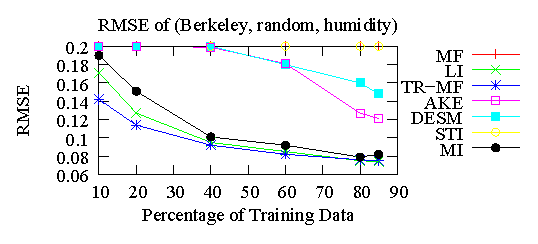
\includegraphics[width=4.4cm, height=2.1cm, trim=15 0 0 0, clip]{table2_1_BRH.eps}
}
\hspace{-0.3cm}
%\end{figure}
%\begin{figure}[H]
%\centering
\subfigure[]
{
	\label{fig:berkeley_random_light}
	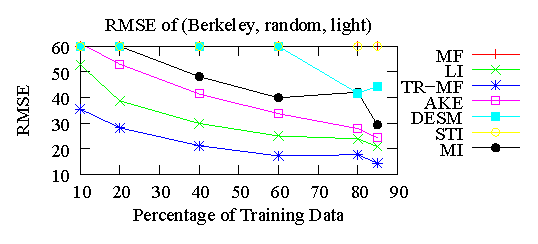
\includegraphics[width=4.4cm, height=2.1cm, trim=15 0 0 0, clip]{table3_BRL.eps}
}
\newline

\hspace{-1cm}
%\caption{}
%\end{figure}
%\begin{figure}[H]
%\centering
\subfigure[]
{
	\label{fig:berkeley_random_tem}
	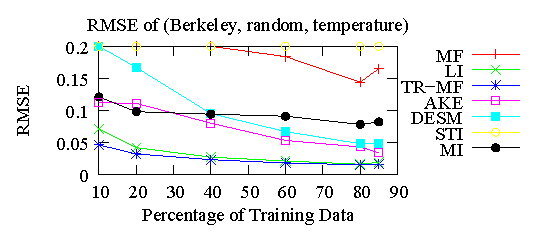
\includegraphics[width=4.4cm, height=2.1cm, trim=15 0 0 0, clip]{table4_BRT.eps}
}
\hspace{-0.3cm}
%\caption{}
%\end{figure}
%\begin{figure}[H]
%\centering
\subfigure[]
{
	\label{fig:traffic_random_hum}
	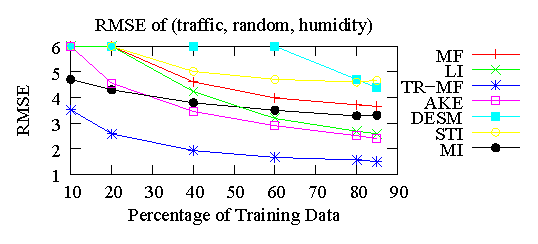
\includegraphics[width=4.4cm, height=2.1cm, trim=15 0 0 0, clip]{table5_TRH.eps}
}
\newline

\hspace{-1cm}
%\caption{}
%\end{figure}
%\begin{figure}[H]
%\centering
\subfigure[]
{
	\label{fig:traffic_random_tem}
	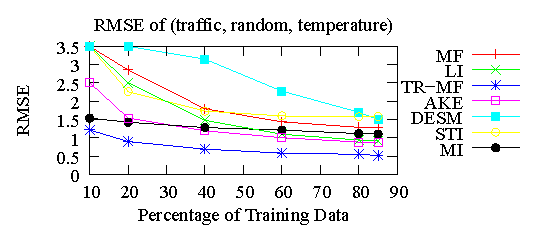
\includegraphics[width=4.4cm, height=2.1cm, trim=15 0 0 0, clip]{table6_TRT.eps}
}
%\caption{Random Split}
\hspace{-0.3cm}
%\caption{}
%\end{figure*}
%\begin{table*}
%%
%\begin{tabular}{cc}
%\subfigure[A]{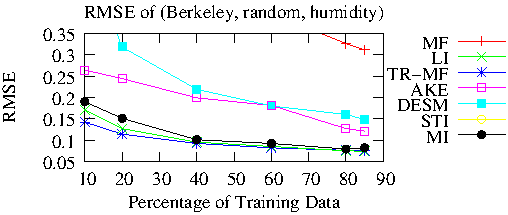
\includegraphics[height=2.5cm, trim=15 0 0 0, clip]{table2_BRH}} 
%   & \subfigure[B]{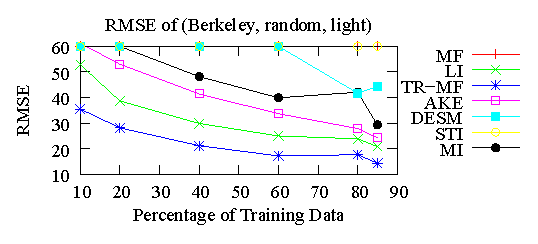
\includegraphics[height=2.5cm, trim=15 0 0 0, clip]{table3_BRL}}\\
%\end{tabularx}
%\end{table*}
%\end{figure}
%\begin{figure}[H]
%\centering
%\mbox{
%\input{table11.pspdftex}}
%\caption{RMSE of (traffic, temporal, temperature}
%\end{figure}
%\begin{figure*}[htbp]
%\centering
\subfigure[]
{
	\label{fig:berkeley_temporal_hum}
	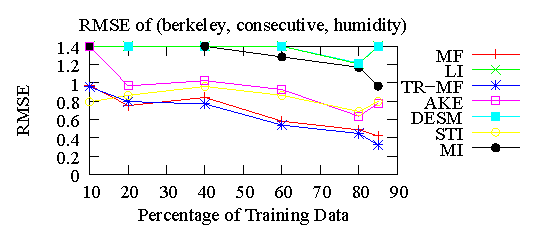
\includegraphics[width=4.4cm, height=2.1cm, trim=15 0 0 0, clip]{table7_BTH.eps}
}
\newline

\hspace{-1cm}
%\end{figure}
%\begin{figure}[H]
%\centering
\subfigure[]
{
	\label{fig:berkeley_temporal_light}
	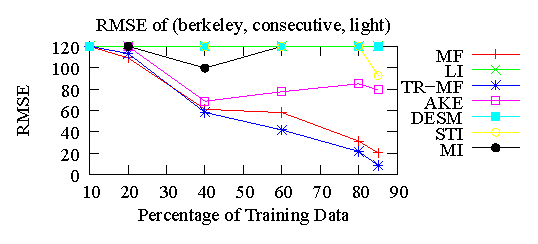
\includegraphics[width=4.4cm, height=2.1cm, trim=15 0 0 0, clip]{table8_BTL.eps}
}
\hspace{-0.3cm}
%\caption{}
%\end{figure}
%\begin{figure}[H]
%\centering
\subfigure[]
{
	\label{fig:berkeley_temporal_tem}
	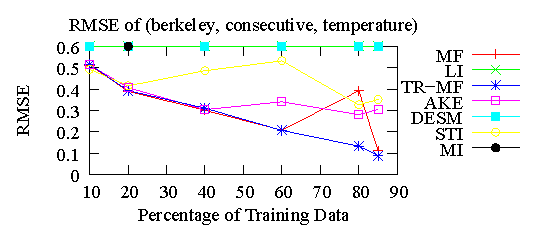
\includegraphics[width=4.4cm, height=2.1cm, trim=15 0 0 0, clip]{table9_BTT.eps}
}
\newline

\hspace{-1cm}
\subfigure[]
{
	\label{fig:traffic_temporal_hum}
	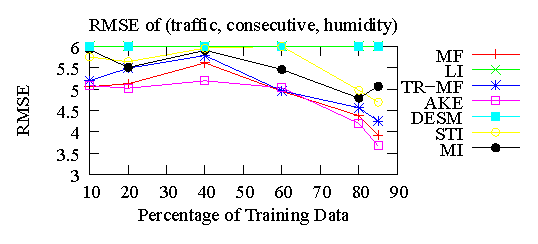
\includegraphics[width=4.4cm, height=2.1cm, trim=15 0 0 0, clip]{table10_TTH.eps}
}
\hspace{-0.3cm}
\subfigure[]
{
	\label{fig:traffic_temporal_tem}
	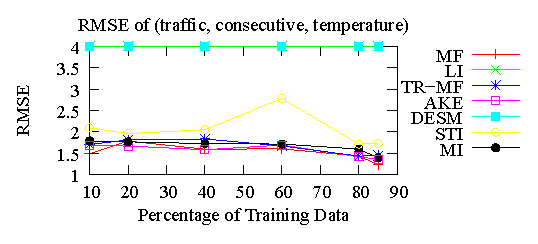
\includegraphics[width=4.4cm, height=2.1cm, trim=15 0 0 0, clip]{table11_TTT.eps}
}
\hspace{0in}

\vspace{-0.3cm}
\caption{Accuracy of salient methods, varying the \newline percentage of training data. (a) to (e) are for \newline
Random Missing data; (f) to (j) are for \newline Consecutive Missing data.}
\hspace{0in}
%\caption{}
\vspace{-1cm}

\end{minipage}

\end{figure}

